% Chapter Template

\chapter{Bidirectional Grounding of Real Data} % Main chapter title

\label{Chapter6} % Change X to a consecutive number; for referencing this chapter elsewhere, use \ref{ChapterX}

\lhead{Chapter 6. \emph{Bidirectional Grounding of Real Data}} % Change X to a consecutive number; this is for the header on each page - perhaps a shortened title

%----------------------------------------------------------------------------------------
%	SECTION 1
%----------------------------------------------------------------------------------------
\section{The Difficulties of Real Data}
In the previous chapter I showed that it is possible to use a \ac{MAE} to bidirectionally ground natural language (words) and the visual attributes of images of different objects through \ac{MRL}. However, the data used in the previous chapter is artificial and therefore many of the challenges which real data presents are not present in it. 

When working with real images, there are many factors to consider such as lighting changes, perspective changes and camera noise \cite{keller2016analysis}. These factors were not present in the ArtS dataset, so in this chapter I will show how these impact \ac{MRL} for bidirectional grounding.



\begin{figure}[h]
    \centering
    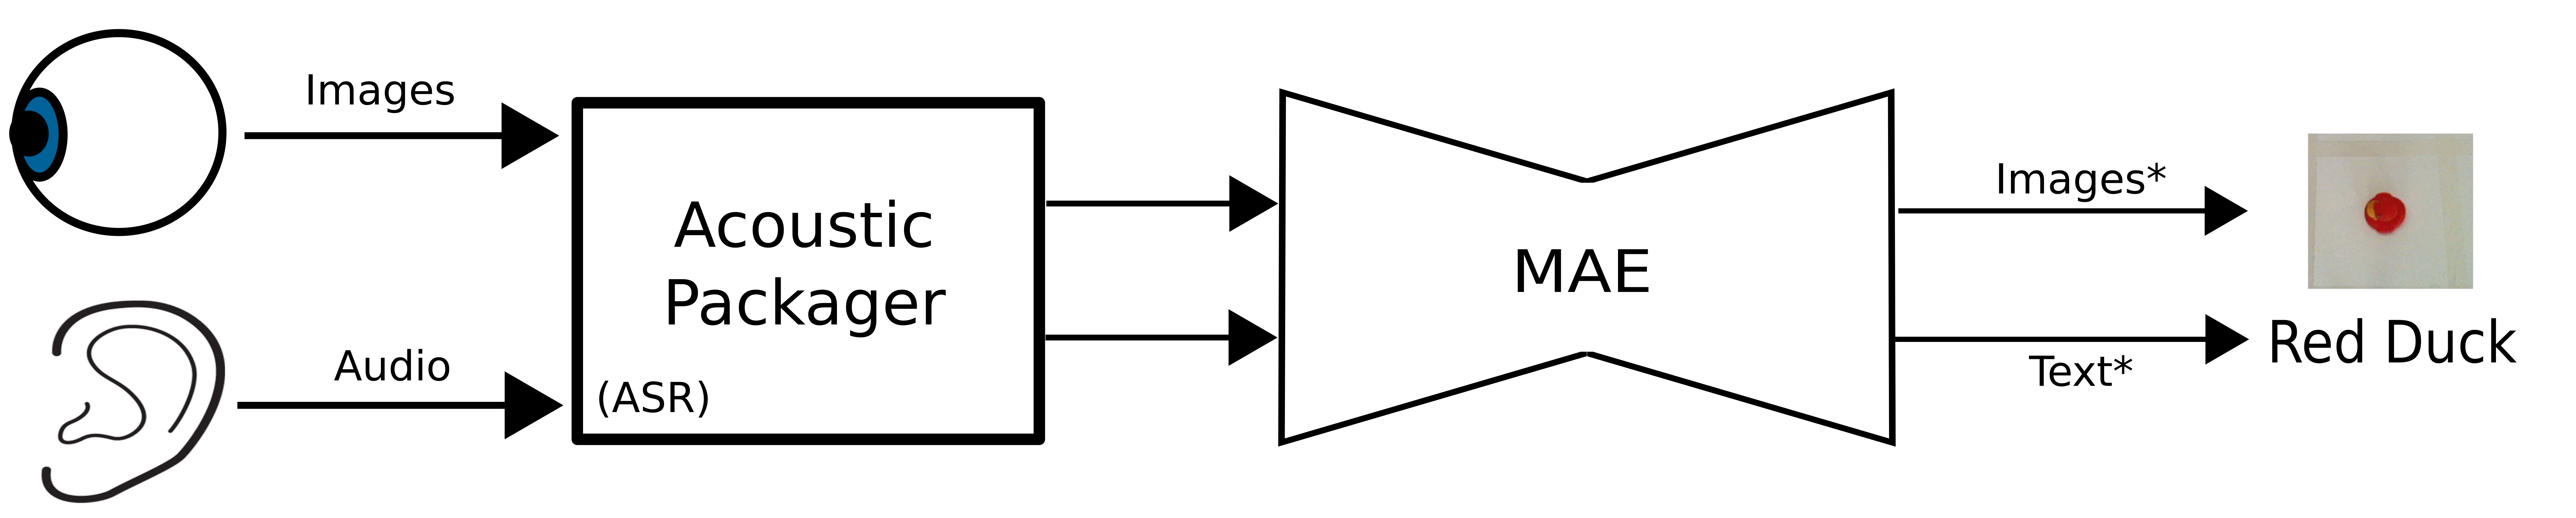
\includegraphics[width=0.7\textwidth]{Figs/chapter6/bimodal_system_schematic.png}
    \caption{System schematic. Data is captured from sensors by an acoustic packager and fed to the multimodal autoencoder.}
    \label{fig:schematic}
\end{figure}

\section{Acoustic Packaging}
In order to make use of \ac{MRL} on a robot, it is necessary to have a method to gather and group data from multiple sensory modalities. To do this, I make use of \ac{AP} \cite{schillingmann2009towards, schillingmann2009computational}.

The acoustic packager I implemented for this, is triggered to capture data when sound above a certain threshold is heard by a microphone. Images and audio are recorded with the audio being passed to an \ac{ASR} system to transcribe any speech. The audio, transcription and image together are refered to as an acoustic-package.

I do not make use of the audio, I use only the transcribed text and images such that the data used in this chapter is analigous to the data used in the previous chapter.

\section{Real Shapes Dataset}

\begin{figure}[h]
    \centering
    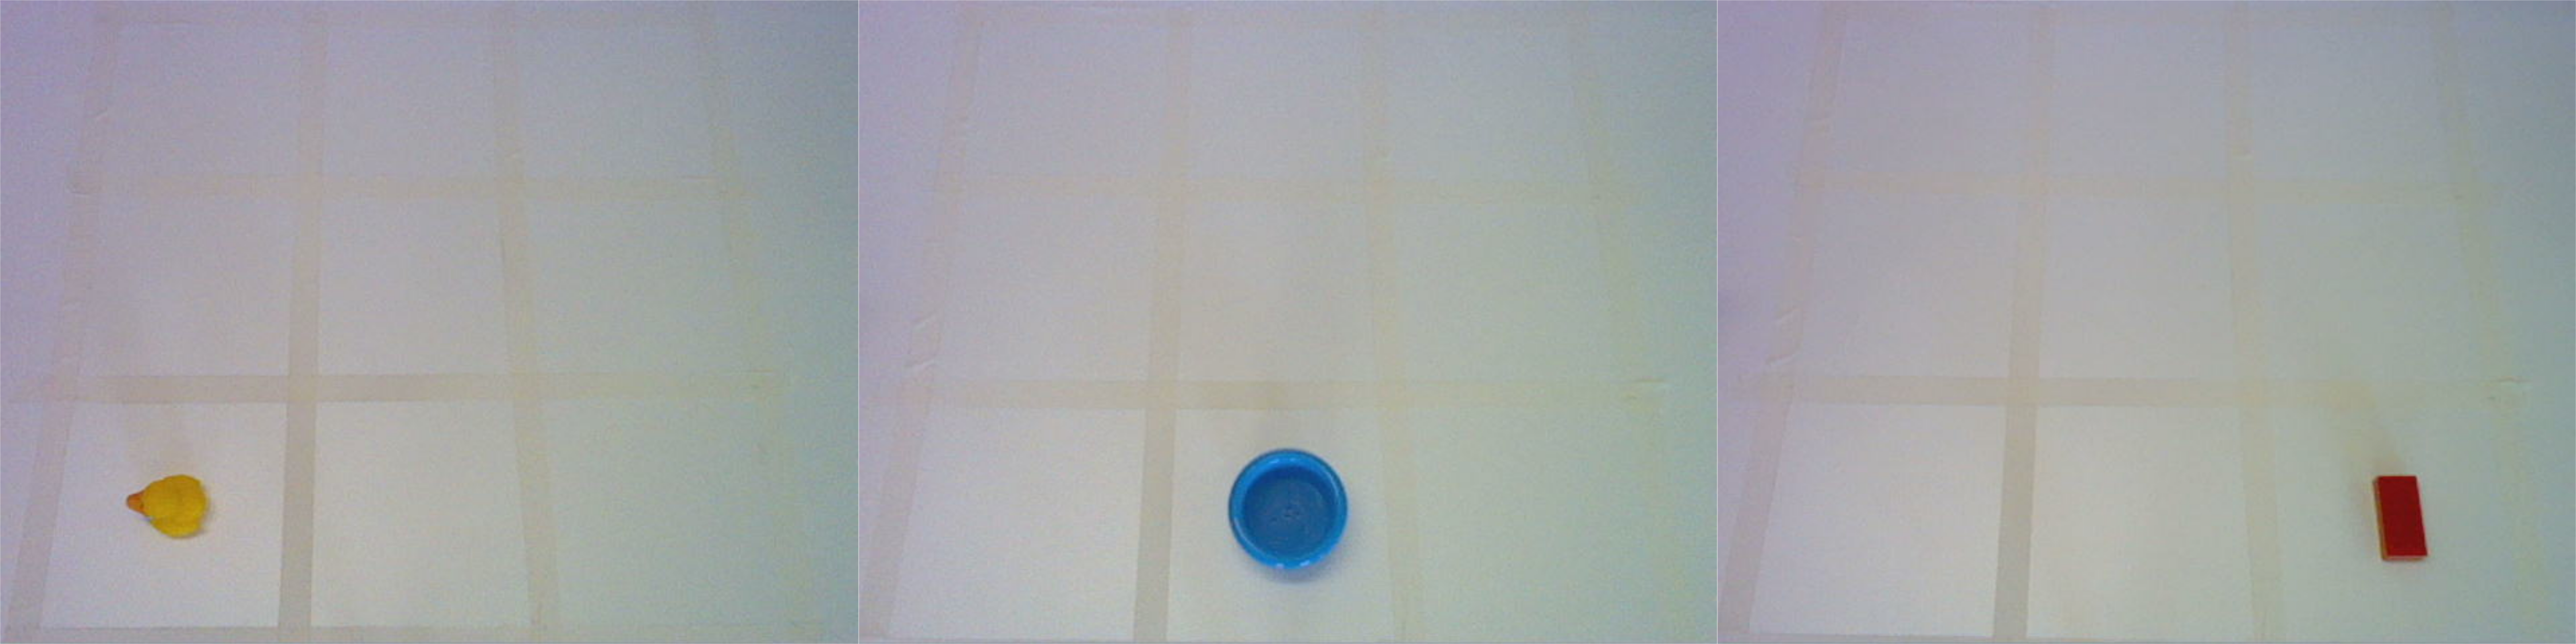
\includegraphics[width=\textwidth]{Figs/chapter6/ReShapeExs.png}
    \caption{Example images from ReShape.}
    \label{fig:ReShape}
\end{figure}

The Real Shapes dataset (ReShape) was created by presenting various objects to a webcam in 9 different positions and giving a short description of the object. \autoref{fig:ReShape} shows example images from ReShape.

\subsection{Dataset Description}
The ReShape dataset contains images and short descriptions of the images.

There are 7 objects, in 10 colours and 3 sizes. Not all objects appear in all 10 colours or all 3 sizes.

\autoref{fig:ReShapeAll} shows cropped, exemplar images for all objects in the ReShape dataset. Not all shape-colour-size combinations are covered in the dataset, hence the large number of blank spaces.

\newpage
\begin{figure}[h!]
    \centering
    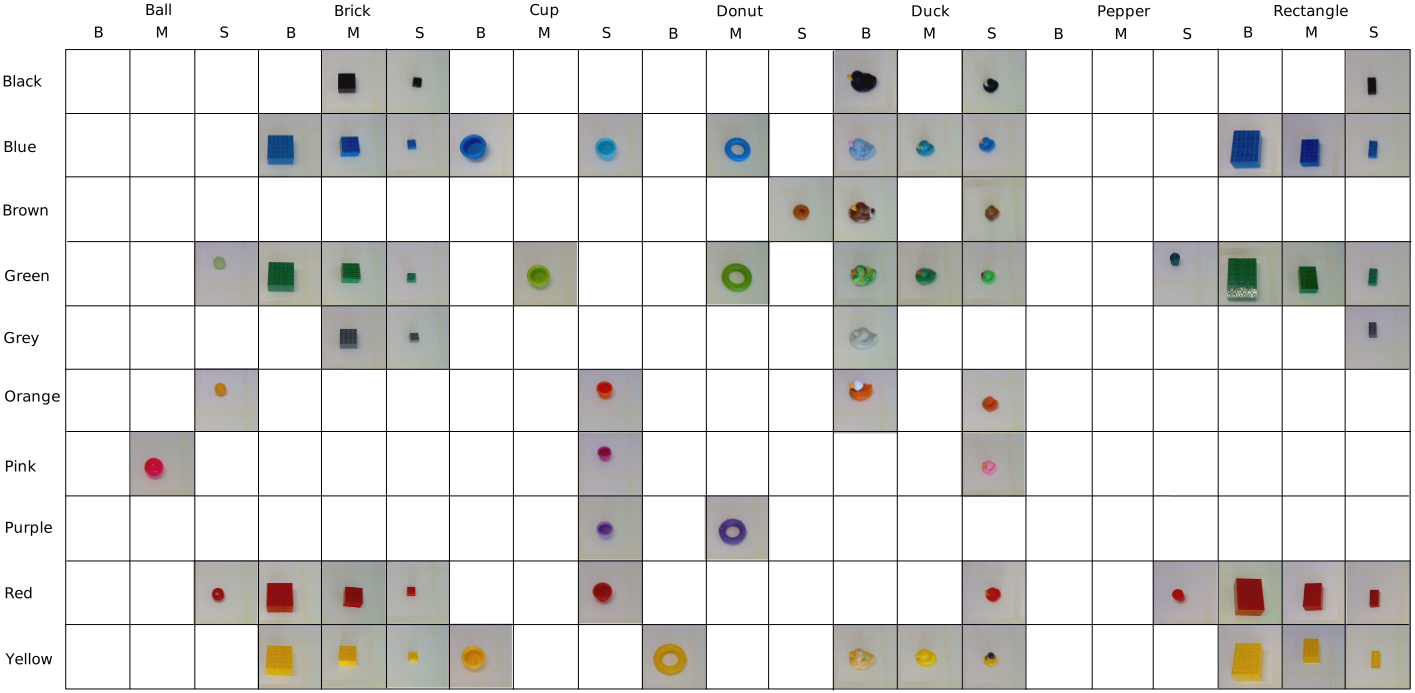
\includegraphics[height=0.7\textwidth, angle=90]{Figs/chapter6/ExemplarAllClasses.png}
    \caption{Exemplar images for all objects in the ReShape dataset.}
    \label{fig:ReShapeAll}
\end{figure}

The dataset was captured in several sessions across multiple days. This is the main source of vairability in the dataset, as different lighting conditions due to weather and time of day has a significant affect on the appearance of images captured by digital cameras \cite{keller2016analysis, keller}\endnote{In \autoref{fig:ReShapeCrop} differences in the lighting conditions are clearly visible with the top left and top centre image having a blue tint.}.


\subsection{Problem Description}
As in the previsous chapter I will be training \acp{MAE} to learn a joint embedding of images and their descriptions. The descriptions only contain a size, shape and colour and not a position as the images are cropped, centring the object in the image, the notion of position is removed from both modalities.

\subsection{Network Description}
I make use of the same network as used in chapter 4 with an embedding size of 296 neurons. 

\section{Experiments with the ReShape dataset}
I will perform two experiments, one with a small subset of the ReShape dataset with complete coverage of every trained and tested combination of colour, object and size is available. The second will make use of a larger variety of objects and colours, however not every combination of object, colour and size is available for training, thus there is not complete coverage, this is similar to experiment 5 in \autoref{Chapter5} where one object-colour combination was excluded from the training data. 

I will also look at the effect of pretraining on the data from experiment 1 and then training for experiment 2. Further to this, two training procedures will be introduced and compared, simple and exemplar.

\subsection{Data Preprocessing}

In the following experiments I do not consider the notion of position and instead crop each image so that the object is roughly centred and consider all objects of the same type to be the equivalent regardless of position (e.g. a \textsc{big blue duck top left} is considered the same as a \textsc{big blue duck center}). As such, the position word is removed from the description of the image and the \ac{MAE} does not contain the position words in its "vocabulary".

\begin{figure}[h]
    \centering
    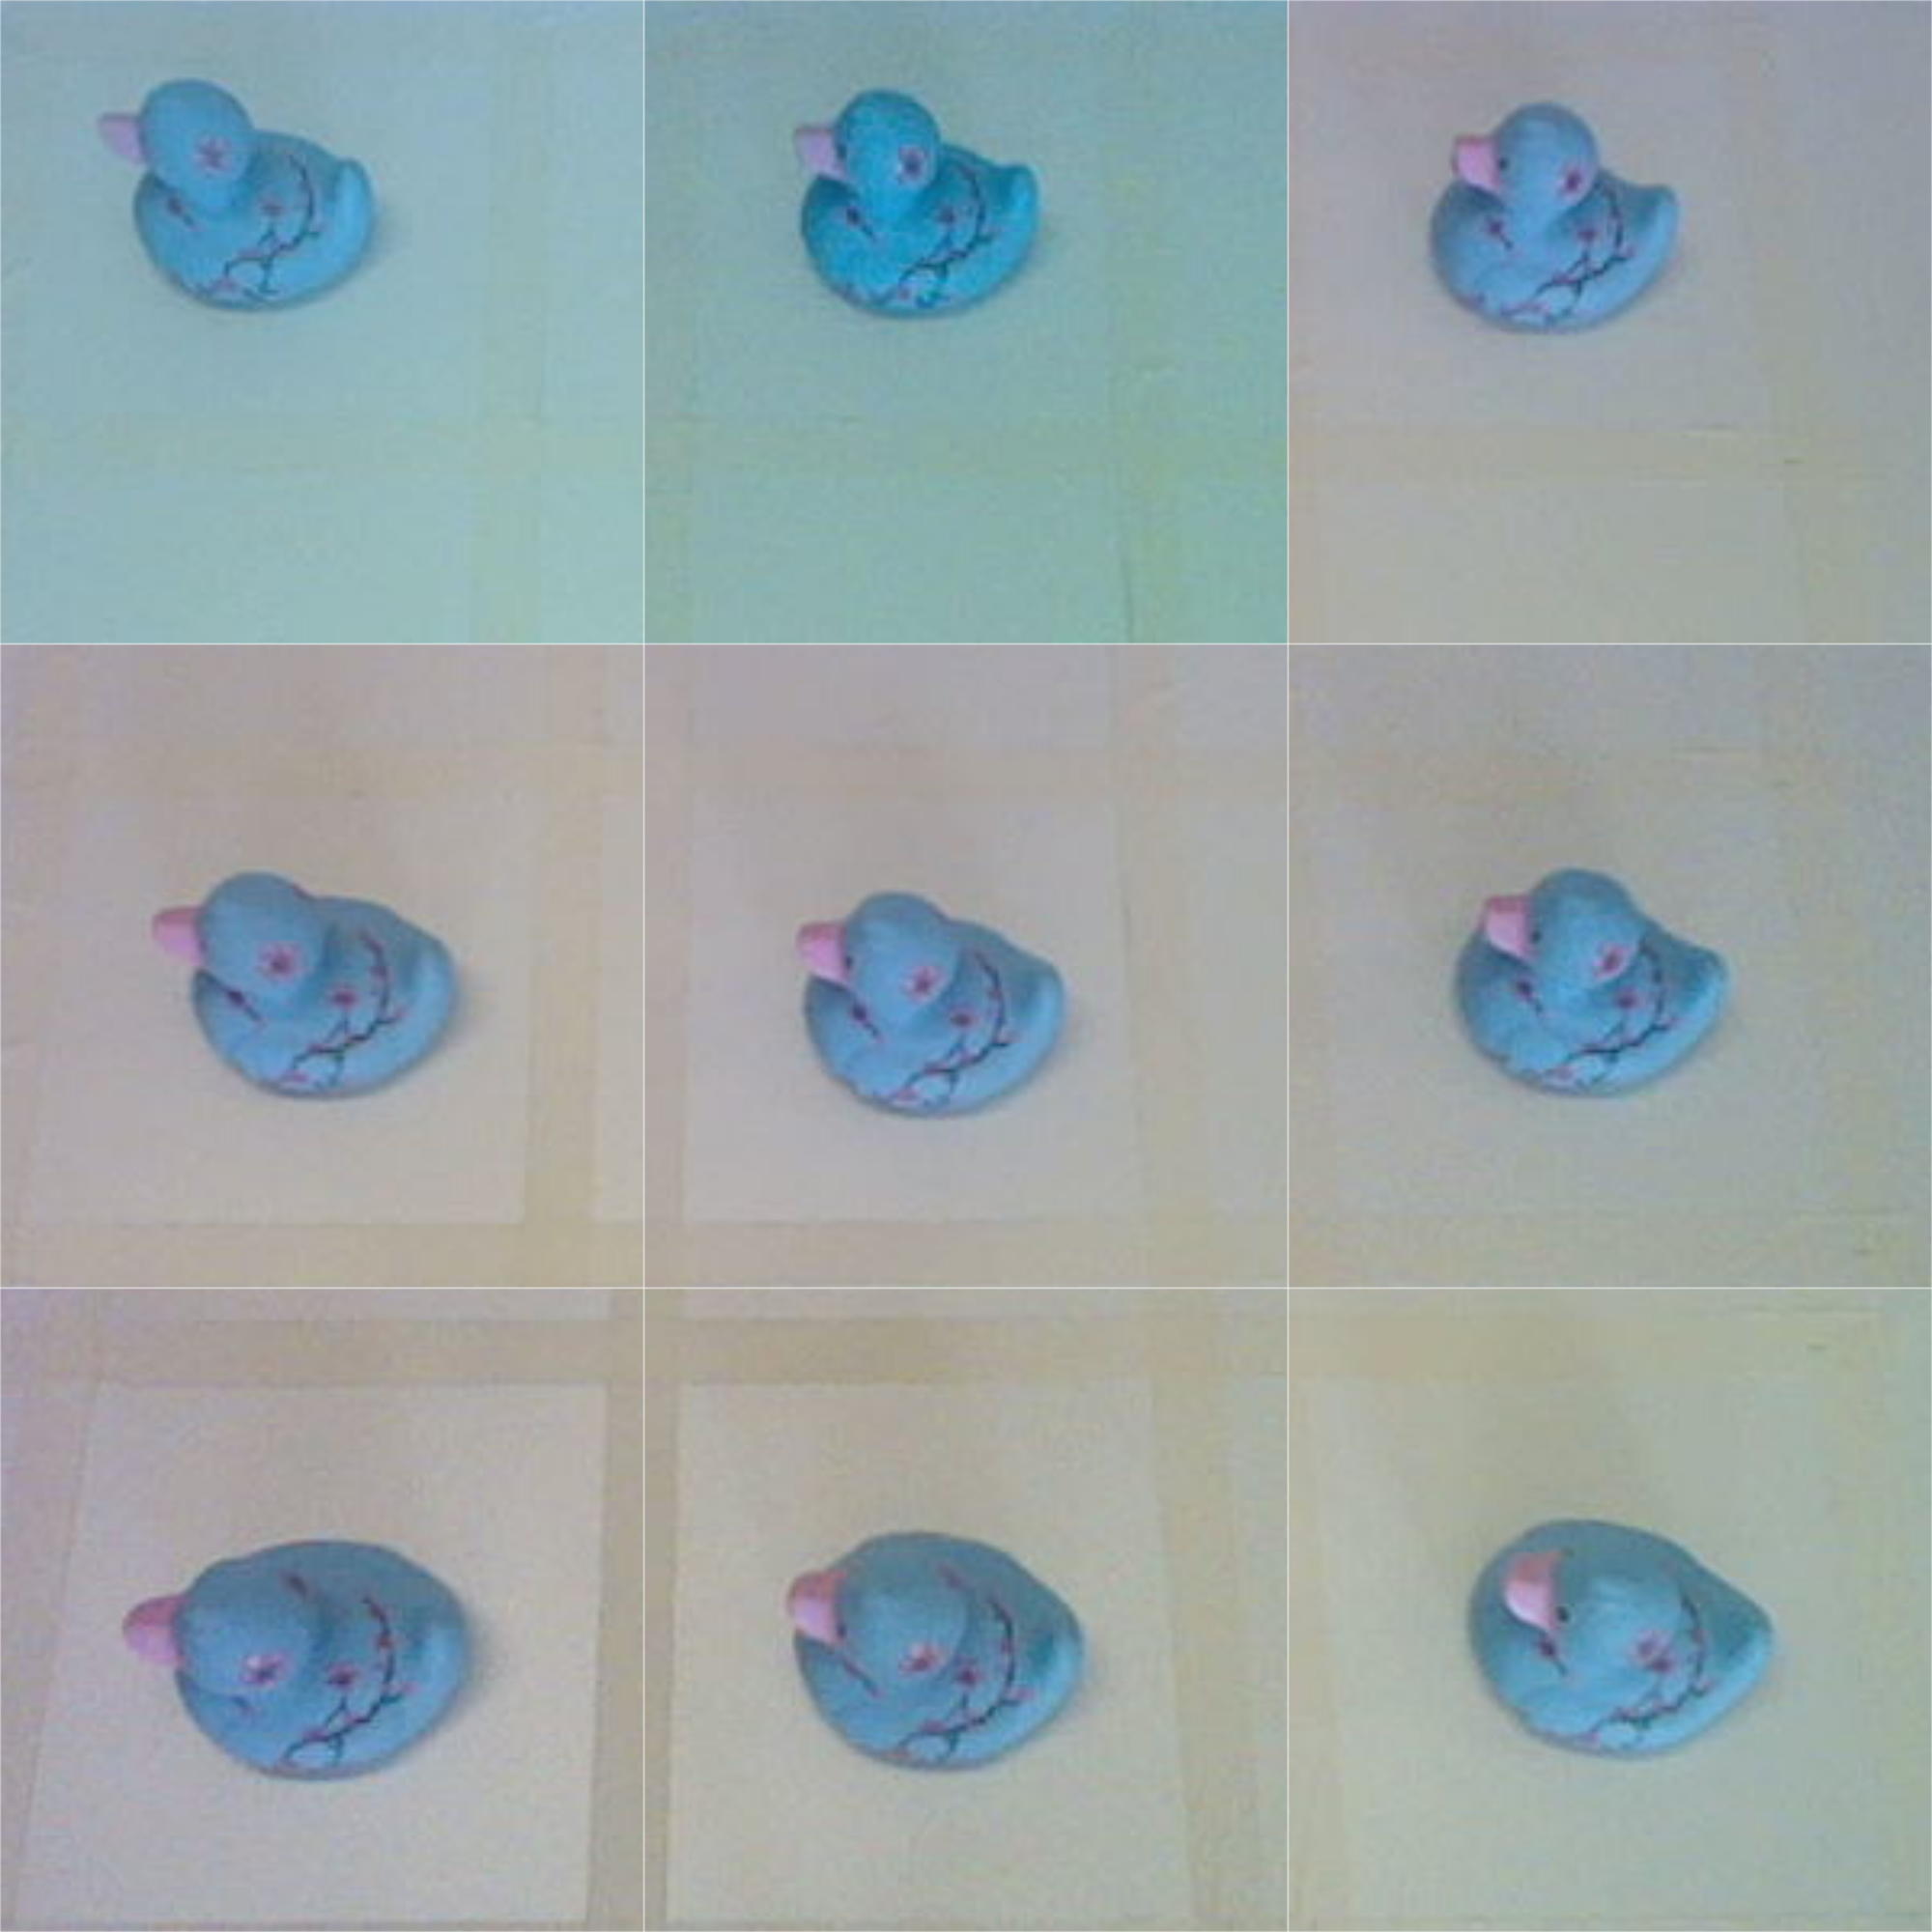
\includegraphics[width=0.7\textwidth]{Figs/chapter6/ReShapeCrop.png}
    \caption{Example cropped images from ReShape.}
    \label{fig:ReShapeCrop}
\end{figure}

Cropping the images is done for three main reasons. 1) this increases the amount of training data for each object by a factor of nine. As the notion of position is removed, the same object in a different position is no longer considered a separate object (unlike in the previous chapter). 2) Cropping reduces the amount of the \ac{MAE}'s field of view which contains the background. This makes it easier for the \ac{MAE} to learn the visual attributes of the objects as less computation is wasted processing the background. 3) Cropping greatly reduces the necessary computation to process a single image as the images are much smaller. Cropping does this without reducing the size of the object in the image unlike resizing the raw image.

Cropping is performed heuristicly, using the position word from the image description to crop out a predefined region. \autoref{fig:CropHeur} shows the regions that each position word relates to for the purposes of cropping.

\begin{figure*}[ht]
    \centering
    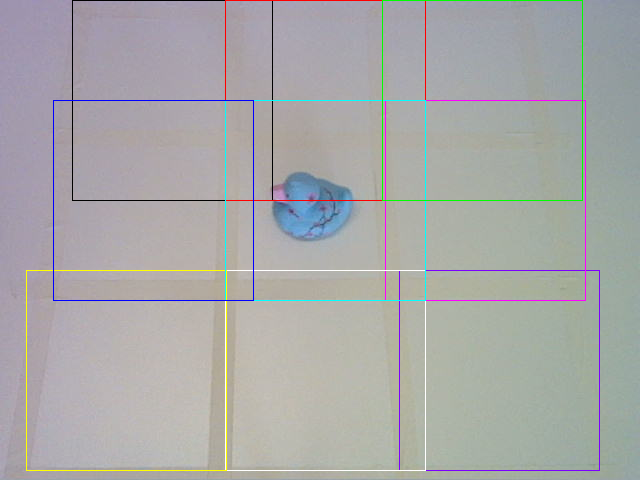
\includegraphics[width=0.7\textwidth]{Figs/chapter6/cropHeuristics.png}
    \caption{Regions to crop to given different postion words.}
    \label{fig:CropHeur}
\end{figure*}


%After cropping, their are changes in the visual attributes of the images which are not accounted for in their descriptions. For example, images in top positions, were further from the camera so they appear slightly smaller than those in bottom positions.

\subsection{Training Procedures}

Calculating the average image for each object provides insight into what to expect when generating images in the Words Only test condition.


\begin{figure*}[ht]
    \centering
    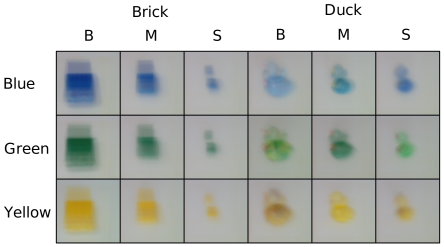
\includegraphics[width=0.7\textwidth]{Figs/chapter6/avgBrickDuckBGY.png}
    \caption{Exp 1: Average of the training images of bricks and ducks in different sizes and colours.}
    \label{fig:AvgBrickDuck}
\end{figure*}

\begin{figure*}[ht]
    \centering
    \includegraphics[width=\textwidth]{Figs/chapter6/avgMost.png}
    \caption{Exp 2: Average of the training images for bricks, cups, donuts, ducks, and rectangles, in different sizes and colours.}
    \label{fig:avgMost}
\end{figure*}

The simple training procedure has the MAE trained to optimise the \ac{MSE} of its output with respect to all of the training data. In the Words Only test condition, the ``best'' images for it to generate are therefore the average images for each object. \autoref{fig:AvgBrickDuck} shows the average image for each object used in experiment 1. \autoref{fig:avgMost} shows the average image for each object in experiment 2.

As the average images are very blurry, it would be useful to have a method which would cause the \ac{MAE} to produce better quality images so that it is easier to inspect which of the visual attributes it has learned to generate correctly.

Using the exemplar training procedure I replace the training image targets with exemplars for each class, when only words are provided as input.

Exemplars are selected by first calculating the average image for each object (\autoref{fig:AvgBrickDuck}, \ref{fig:avgMost}). I then select the training image with the smallest \ac{MSE} from the average image for each object to be the exemplar for that object. 

\autoref{fig:ExmBrickDuck} shows the exemplars used in experiment 1 and \autoref{fig:ExmMost} shows the exemplars for experiment 2.

\begin{figure*}[ht]
    \centering
    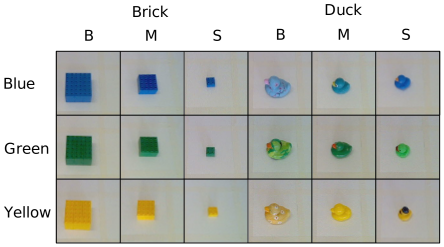
\includegraphics[width=0.7\textwidth]{Figs/chapter6/avgBrickDuckBGYExemplars.png}
    \caption{Exp 1: Exemplar images of bricks and ducks in different sizes and colours.}
    \label{fig:ExmBrickDuck}
\end{figure*}


\subsection{Experiment 1}
Experiment 1 makes use of two shapes in three colours and three sizes. The shapes and colours were selected as they are the only shape-colour combinations that occur in all three sizes in the dataset.

\begin{table}[h]
\centering
\begin{tabular}{|c|c|c|}
\hline

\textbf{Shapes}  & \textbf{Colours} & \textbf{Sizes}\\ \hline \hline
Brick  & Yellow  & Big \\ \hline
Duck   & Green   & Medium \\ \hline
& Blue & Small \\ \hline
			  
			
\end{tabular}
\caption{Experiment 1 data subset.}
\label{tab:6_exp1_data} 
\end{table}


\subsubsection{Results}

Overall, the \ac{MAE} has similar performance in terms of \ac{MSE} using both the simple and exemplar training procedures. Whilst the exemplar method lead to slightly better performance in the Bimodal and Image Only test conditions, this is traded off for worse performance in the Words Only condition. The fact that the \ac{MSE} in the Words only condition is small, shows that the mean image for the training and testing data is very similar.

\begin{table}[h!]
\centering
	\begin{tabular}{|c|c|c|c|}
	\hline
\textbf{Training} & 	\textbf{Bimodal} & 	\textbf{Image Only} 	& 	\textbf{Words Only} \\ \hline
Simple & 2.14 $\mypm$ 0.11 & 4.00	$\mypm$ 0.04 & 6.02 $\mypm$ 	0.01 \\ \hline
Exemplar & 2.06 $\mypm$ 0.07 & 3.44 $\mypm$ 0.51 & 7.92	$\mypm$ 0.02 \\ \hline
\end{tabular}
\caption{Exp 1: Total Mean Squared Error for different test conditions and training procedures. (All values are $\times10^{-3}$.)}
\label{tab:6_res_exp1}
\end{table}

The similarity between the training and test data is expected in this case as the dataset was created using the same set of objects, in the same location on the same background. As previously mentioned, the main source of variability in the dataset is caused by changes in lighting conditions across the different data-capture sessions. However, this demonstrates an issue with using \ac{MSE} as the cost function to train the \ac{MAE}. If a different example of an object, captured on a different background, from a different angle is used to test the \ac{MAE}, the \ac{MSE} will be very high in the Words Only condition as this image will be very far from the mean image of the training data.

The addition of more training data, with more diverse examples and more detailed descriptions should help. However, as the system is designed for operation on a robot, its absolute performance on a dataset isn't really that important. It is of more worth that the \ac{MAE} generate a "big blue duck" when asked to, than to generate the specific "big blue duck" the user had in mind.

\paragraph{Image Generation}

Comparing \autoref{fig:simpleGen_1} and \autoref{fig:AvgBrickDuck} it can be seen that the generated images are almost identical to the average training images for each description when the Simple training procedure is used. 

\begin{figure*}[ht]
    \centering
    \includegraphics[width=0.7\textwidth]{Figs/chapter6/avgBrickDuckBGYGenerated.png}
    \caption{Exp 1: Images generated from full descriptions using the \ac{MAE} trained with the simple procedure.}
    \label{fig:simpleGen_1}
\end{figure*}

Similarly, the Exemplar images from \autoref{fig:ExmBrickDuck} and the images generated by the Exemplar \ac{MAE} in \autoref{fig:exemplarGen_1} are also almost identical.

\begin{figure*}[ht]
    \centering
    \includegraphics[width=0.7\textwidth]{Figs/chapter6/avgBrickDuckBGYGeneratedExemplars.png}
    \caption{Exp 1: Images generated from (only) full descriptions using the MAE trained with the exemplar procedure.}
    \label{fig:exemplarGen_1}
\end{figure*}

These two results show that the \ac{MAE} has overfitted the training data, however this isn't necessarily a bad thing as the generated images are correct for the input descriptions and the \ac{MAE} has perfect accuracy at labelling the test data in the Image Only condition (\autoref{tab:6_res_exp1_acc}).



\begin{figure*}[ht]
    \centering
    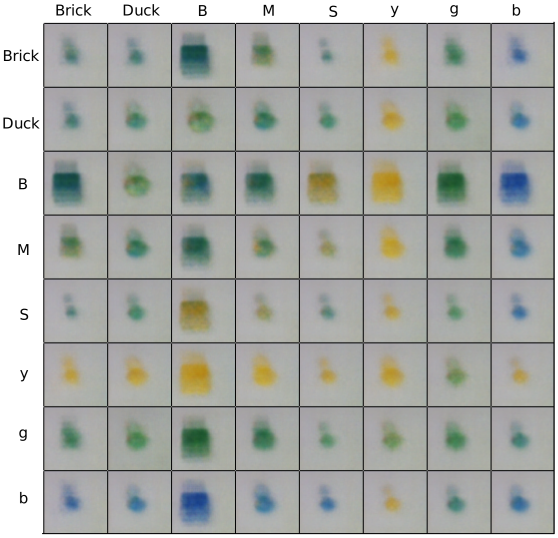
\includegraphics[width=0.7\textwidth]{Figs/chapter6/2wordsSimpleBrickDuck.png}
    \caption{Exp 1: Images generated using word pairs using the MAE trained with the simple procedure.}
    \label{fig:2wordsSimpleBrickDuck}
\end{figure*}

\begin{figure*}[ht]
    \centering
    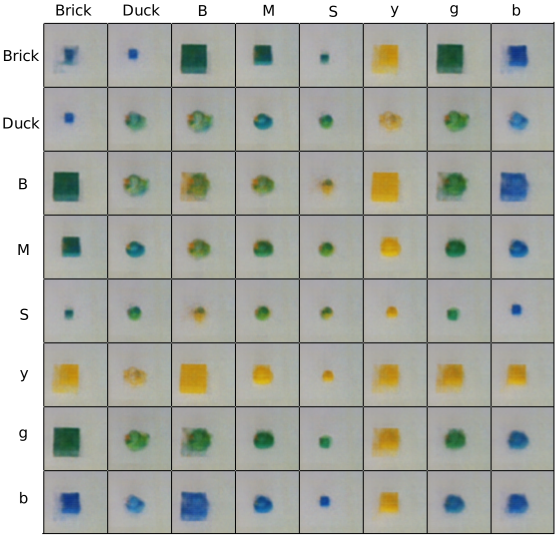
\includegraphics[width=0.7\textwidth]{Figs/chapter6/2wordsExemplarBrickDuck.png}
    \caption{Images generated using word pairs using the MAE trained using image exemplars. (Only words are provided as input.)}
    \label{fig:2wordsExemplarBrickDuck}
\end{figure*}


It is hard to tell how well the \ac{MAE} has learnt the grounded meanings of each individual word when the simple training procedure is used as the generated images are very blurry (\autoref{fig:2wordsSimpleBrickDuck}). The meanings of colours and sizes has been correctly learnt with \textsc{Yellow}, \textsc{Green} and  \textsc{Blue} generating the correct coloured pixels. \textsc{Big} \textsc{Medium} and \textsc{Small} also lead to the correct alteration in number of coloured pixels generated.

In \autoref{fig:2wordsExemplarBrickDuck} as well as the correct grounding of the colours and sizes, we also see that the names of the objects have been correctly grounded, with \textsc{brick} generating a square shape and \textsc{Duck} generating a rubber-duck shape. We also see that detials such as the duck's beak are generated as well as the black top hat on the small yellow duck.

Whilst the generation of the beak is desirable, as all ducks have beaks, the top hat is specific to only two instances of ducks in the training data, a \textsc{big yellow duck} and a \textsc{small yellow duck}. The influence of the top hat can be seen in \autoref{fig:simpleGen_1} with the 
\textsc{big yellow duck} having a black area on its head.

The top hat further highlights that the \ac{MAE} learns to generate the mean image for a given object. So, as with the blurring of the images cuased by the simple training procedure and remedied by the exemplar procedure, is there a method to reduce the introduction of training data specific artifacts like the top hat?

The simplest method to deal with this, would be to increase the complexity of the descriptions of the images. If the duck with a top hat were referred to as "big yellow duck with a top hat", which could be encoded to the network as \textsc{big yellow duck black top hat} by expanding its vocabulary, then distinguishing whether to generate an image of a duck with or without a top hat would be simple.


\paragraph{Multilabel Classification}

The \ac{MAE} achieves 100\% accuracy on description generation across all three test conditions. This suggests that the test data has a very similar distribution to the training data. As the test data is images of the same objects captured in the same environment, the only differences between the training data and test data will be small changes in object position and  changes in lighting as the test data was captured on a different day and at a different time of day. Thus, the mean image from the training data for each object is likely very close to the mean image for each object in the test data respectively. It is unlikely that such good performance would be achieved with even small changes to viewing angle or background, which are both constant across the training and test data. However, the addition of more diverse training examples would also alleviate this \cite{keller2016analysis, keller}.


\begin{table}[h!]
\centering
	\begin{tabular}{|c|c|c|c|}
	\hline
\textbf{Training }	 & 	\textbf{Bimodal} & \textbf{Image Only} 	& 	\textbf{Words Only} \\ \hline
Simple & 100.00 $\mypm$ 0.00 & 100.00 $\mypm$ 0.00 & 100.00 $\mypm$ 0.00 \\ \hline
Exemplar & 100.00 $\mypm$ 0.00 & 100.00 $\mypm$ 0.00 & 100.00 $\mypm$ 0.00 \\ \hline
	\end{tabular}
\caption{Exp 1: Percentage Description Accuracy for different test conditions and training procedures.}
\label{tab:6_res_exp1_acc}
\end{table}


\subsection{Experiment 2}

Experiment 2 makes use of five shapes in five colours and three sizes. The additional shapes and colours were selected as they are represented in most sizes in the dataset.

\begin{table}[h]
\centering
\begin{tabular}{|c|c|c|}
\hline

\textbf{Shapes}  & \textbf{Colours} & \textbf{Sizes}\\ \hline \hline
Brick  & Yellow  & Big \\ \hline
Duck   & Green   & Medium \\ \hline
Donut & Blue & Small \\ \hline
Cup  & Red & \\ \hline
Rectangle & Black & \\ \hline

\end{tabular}
\caption{Experiment 2 data subset.}
\label{tab:6_exp2_data} 
\end{table}

\begin{figure*}[ht]
    \centering
    \includegraphics[width=\textwidth]{Figs/chapter6/exemplarMost.png}
    \caption{Exp 2: Exemplar images of bricks, cups, donuts, ducks, and rectangles, in different sizes and colours.}
    \label{fig:ExmMost}
\end{figure*}


\subsubsection{Results}

\begin{table}[h!]
\centering
	\begin{tabular}{|c|c|c|c|}
	\hline
\textbf{Training} & 	\textbf{Bimodal} & 	\textbf{Image Only} 	& 	\textbf{Words Only} \\ \hline
Simple &  2.14 $\mypm$	0.07 & 3.89 $\mypm$	0.62 & 6.08 $\mypm$ 0.01 \\ \hline
Exemplar & 2.30 $\mypm$ 0.07 & 3.67 $\mypm$ 0.23
& 10.51	$\mypm$ 0.01 \\ \hline

\end{tabular}
\caption{Exp 2: Total Mean Squared Error for different test conditions and training procedures. (All values are $\times10^{-3}$.)}
\label{tab:6_res_exp2}
\end{table}


\subsubsection{Image Generation}

The \ac{MAE} is able to generalise to unseen combinations of attributes, confirming the result found in the final experiment of the previous chapter (Experiment 5 \autoref{Chapter5}). However, in this case, we have many more missing examples. \autoref{fig:mostExemplarGen} shows the images generated from full descriptions by the \ac{MAE} trained using exemplars. The red borders show images which have exemplars; those without red borders are not seen in the training data, yet the \ac{MAE} is still able to produce good approximations of these objects.

\begin{figure*}[ht]
    \centering
    \includegraphics[width=\textwidth]{Figs/chapter6/exemplarMostGenerated.png}
    \caption{Exp 2: Images generated from full descriptions using the \ac{MAE} trained with the exemplar procedure. Red borders show objects with exemplar images.}
    \label{fig:mostExemplarGen}
\end{figure*}

The clearest example of generalisation to unseen objects is the generation of donuts in \autoref{fig:mostExemplarGen}. Despite only having 3 examples of donuts, the \ac{MAE} is able to generate images of donuts in different colours and sizes.  

The quality of the generated images for unseen objects is strongly linked to whether there is a similar example to the requested image. For example, the \textsc{big green donut} and \textsc{small green donut} are of a higher quality than the \textsc{big red donut} and \textsc{small red donut}. This is due to the existence of a \textsc{medium green donut} in the training data. As there are no red donuts in the training data, the \ac{MAE} must rely on its knowledge of the meanings of the individual words \textsc{big}, \textsc{red} and \textsc{donut} to generate an image of a \textsc{big red donut}. For the \textsc{big green donut}, the \ac{MAE} has an example of a \textsc{medium green donut} so it must only alter the size of the object in the image, it does not need to generate the image from the individual words \textsc{big}, \textsc{green} and \textsc{donut}.

In general the \ac{MAE} shows its worst performance on \textsc{black} objects, this is likely due to the reletively few examples of black objects in the training data (5 for black versus 8 for red, 11 for green, 11 for yellow and 12 for blue).

\begin{figure*}[ht]
    \centering
    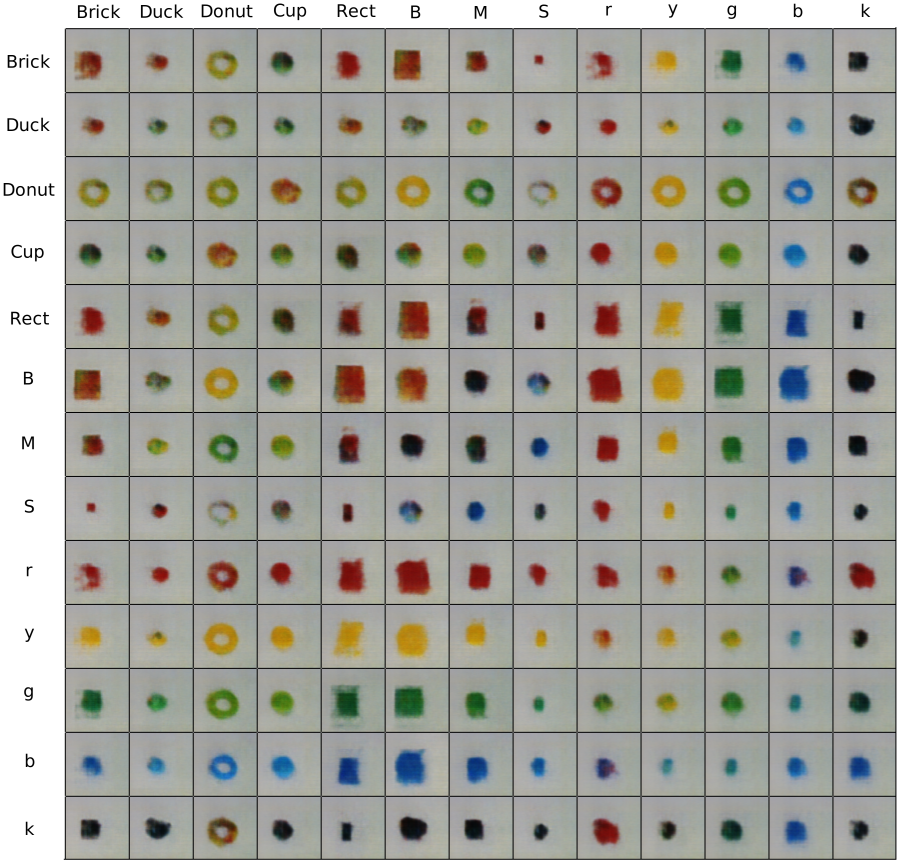
\includegraphics[width=\textwidth]{Figs/chapter6/2wordsMostExemplar.png}
    \caption{Exp 2: Images generated using word pairs using the \ac{MAE} trained using image exemplars when only words are provided as input.}
    \label{fig:2wordsMostExemplar}
\end{figure*}


In \autoref{fig:2wordsMostExemplar} we can see the output of the \ac{MAE}'s image output when only two words are given as input. The meaning of the different colours has been learnt with all images in the red (r), yellow, (y) green (g) blue (b) and black (k) rows and columns having their appropriate colour except when two colours are given as input (e.g. "yellow green") which does not have a true meaning in this instance. We do however see that some colours are more dominant than others, (in order, y, g, b, r, k), this is likely due to their prominence in the dataset, with more examples of yellow, green and blue objects than either red or black objects. 

Yellow dominating over blue and green is likely due to less variance in the shade of yellow in the dataset vs the variance in shades of blue and green (similarly for green dominating over blue). This can be seen clearly in \autoref{fig:ExmMost} where nearly all of the yellow objects have the same shade of yellow compared to blue where there is a spectrum of blues from dark to light blue.

The sizes have been correctly learnt with big (B) images having more coloured pixels than medium (M) images which in turn have more coloured pixels than small (S) images.

The different shapes have been learnt to different degrees. For example, the Donut is clearly a ring in all valid cases (i.e. when only one object name is provided as input).



\paragraph{Multilabel Classification}

In \autoref{tab:6_res_exp2} we can see the total \ac{MSE} for generation of images and text in the three different test conditions. In all three condition the \ac{MSE} is very low and has low variance across the four cross validation trials.

\paragraph{Description Accuracy}
\begin{table}[h!]
\centering
	\begin{tabular}{|c|c|c|c|}
	\hline
\textbf{Training}	 & 	\textbf{Bimodal} & \textbf{Image Only} 	& 	\textbf{Words Only} \\ \hline
Simple &  100.00 $\mypm$ 0.00 & 100.00 $\mypm$ 0.00 & 100.00 $\mypm$ 0.00 \\ \hline
Exemplar & 100.00 $\mypm$ 0.00 & 100.00 $\mypm$ 0.00 & 100.00 $\mypm$ 0.00 \\ \hline
\end{tabular}
\caption{Accuracy}
\label{tab:6_res_exp2_acc}
\end{table}


In all three test conditions the \ac{MAE} correctly generates descriptions with 100\% accuracy (\autoref{tab:6_res_exp2_acc}. This is due to the similarity of the training and test data, as previously discussed.

\subsection{Discussion}

Applying \ac{MRL} to real data presents many new challenges as compared to when it is applied to the ArtS dataset. Whilst real images have much more noise in them than artificially generated images, the more important difference between Arts and ReShape is that there are many visual attributes in the ReShape dataset which are not accounted for in the image descriptions.

This showed up as the introduction of image artifacts such as the top hat on the yellow duck in both experiments 1 and 2 as well as the blurring of images generated when class exemplars were not used in training. In the ArtS dataset each object was fully described by its description, whereas in ReShape, there are changes in perspective due to the different locations which images were captured at and visual textures such as patterns on the ducks beyond their primary colour (for example, the duck in \autoref{fig:CropHeur} has a floral pattern but is only described as a \textsc{Big Blue Duck}).

There is also the issue of not having full coverage of every size, colour and shape combination. Whilst \ac{MRL} has been demonstrated to cope well with missing examples, correctly generating images of unseen objects, these images are lower quality than the images generated for objects which have exemplars. The fewer examples of a particular shape, colour or size, the worse the image generation for that attribute. \autoref{fig:mostExemplarGen} highlights this, where \textsc{big black donut} is generated as a \textsc{big brown/yellow donut} as the MAE does not have a strong representation of the colour black and only has three examples of donuts.



\section{Summary}
This chapter focused on how \ac{MRL} could be applied to real data, demonstrating how it can be used to solve the symbol grounding problem in an unsupervised manner.
To that end, I have demonstrated that \ac{MRL} can be used to perform bidirectional grounding of images and text. Further to this, I have shown that \ac{MRL} can generalise to unseen examples, correctly generating images of unseen objects.

The ability of the \ac{MAE} to generate images of unseen objects like the \textsc{Big Red Donut} is very exciting. This result hints at the possibility to develop grounded models capable of understanding more diverse visual attributes and larger numbers of objects.

These experiments present a starting point from which more powerful models can be built through the use of larger datasets as well as through the incorporation of advanced  \ac{ANN} techniques such as dilated and multiscale convolutions, and residual connections. The addition of these types of features to the \ac{MAE} architecture could allow for stronger models of image feature scale and shape and how these relate to the words which describe them.

Further discussion of the results from this chapter has been published in \cite{sheppard2020multimodal}.
\theendnotes